\documentclass[12pt,a4paper]{article}

% ── Geometry & spacing ──────────────────────────────────────
\usepackage[margin=2.5cm]{geometry}
\setlength{\headheight}{14.5pt}
\addtolength{\topmargin}{-2.5pt}
\setlength{\parindent}{1.25em}
\setlength{\parskip}{0pt}

% ── Encoding & language ─────────────────────────────────────
\usepackage[T1]{fontenc}
\usepackage[utf8]{inputenc}
% Swap the two lines below to switch language:
% \usepackage[english]{babel}       
\usepackage[indonesian]{babel}     % Bahasa Indonesia

% ── Font ────────────────────────────────────────────────────
\usepackage{lmodern}

% ── Math ────────────────────────────────────────────────────
\usepackage{amsmath, amssymb, amsthm}
\usepackage{mathtools}

% ── Graphics & figures ──────────────────────────────────────
\usepackage{graphicx}
\usepackage{float}
\usepackage{caption}
\usepackage{subcaption}
\graphicspath{{doc/}}

% ── Tables ──────────────────────────────────────────────────
\usepackage{booktabs}
\usepackage{array}
\usepackage{longtable}

% ── Lists ───────────────────────────────────────────────────
\usepackage{enumitem}

% ── Code listings ───────────────────────────────────────────
\usepackage{listings}
\usepackage{xcolor}

\definecolor{codebg}{RGB}{245,245,245}
\definecolor{codeframe}{RGB}{200,200,200}
\definecolor{codekw}{RGB}{0,0,180}
\definecolor{codecomment}{RGB}{60,128,49}
\definecolor{codestring}{RGB}{163,21,21}

\lstdefinestyle{default}{
  backgroundcolor=\color{codebg},
  basicstyle=\ttfamily\small,
  breaklines=true,
  breakatwhitespace=false,
  tabsize=2,
  showstringspaces=false,
  frame=single,
  rulecolor=\color{codeframe},
  numbers=left,
  numberstyle=\tiny\color{gray},
  numbersep=8pt,
  xleftmargin=2.5em,
  framexleftmargin=2em,
  keywordstyle=\color{codekw}\bfseries,
  commentstyle=\color{codecomment}\itshape,
  stringstyle=\color{codestring},
}
\lstdefinestyle{go}{style=default, language=Python}    % closest builtin
\lstdefinestyle{python}{style=default, language=Python}
\lstdefinestyle{java}{style=default, language=Java}
\lstdefinestyle{cpp}{style=default, language=C++}
\lstdefinestyle{bash}{style=default, language=bash}

\lstset{style=default}   % global default

% ── Boxes (for tips / callouts) ──────────────────────────────
\usepackage{tcolorbox}
\tcbuselibrary{listings, skins, breakable}

\newtcolorbox{infobox}[1][Note]{
  colback=blue!5!white, colframe=blue!50!black,
  fonttitle=\bfseries, title=#1,
  breakable
}
\newtcolorbox{warnbox}[1][Warning]{
  colback=orange!10!white, colframe=orange!80!black,
  fonttitle=\bfseries, title=#1,
  breakable
}

% ── Hyperlinks ──────────────────────────────────────────────
\usepackage{hyperref}
\usepackage{xurl}
\hypersetup{colorlinks=true, linkcolor=black, urlcolor=blue, citecolor=black}

% ── SI units ────────────────────────────────────────────────
\usepackage{siunitx}

% ── Header / Footer ─────────────────────────────────────────
\usepackage{fancyhdr}
\pagestyle{fancy}
\fancyhf{}
\lhead{\CourseCode{} -- \CourseName}
\rhead{\thepage}

% ── First-line indent on all sections ───────────────────────
\usepackage{indentfirst}

\newcommand{\CourseCode}{IF2224}
\newcommand{\CourseName}{Teori Bahasa Formal dan Otomata}
\newcommand{\AssignmentTitle}{Laporan Tugas Besar}
\newcommand{\AssignmentSubtitle}{Milestone 1}
\newcommand{\Semester}{Semester II / 2025--2026}

% Team / group
\newcommand{\GroupName}{GTFOTBFO (HBB)}
\newcommand{\MemberA}{Nathanael Imandatua Manurung - 13524021}
\newcommand{\MemberB}{Nicholas Wise Saragih Sumbayak - 13524037}
\newcommand{\MemberC}{Kurt Mikhael Purba - 13524065}
\newcommand{\MemberD}{Rava Khoman Tuah Saragih - 13524107}


% Institution
\newcommand{\Lab}{Laboratorium Ilmu dan Rekayasa Komputasi}
\newcommand{\Program}{Teknik Informatika}
\newcommand{\Faculty}{Sekolah Teknik Elektro dan Informatika}
\newcommand{\University}{Institut Teknologi Bandung}

% Repository link (used in Appendix)
\newcommand{\RepoURL}{https://github.com/nicholaswisee/HBB-Tubes-IF2224-2026}
\newcommand{\DeployURL}{https://your-deployment-url.example.com}
\newcommand{\DFAURL}{https://drive.google.com/file/d/1XT-esS_K76ImoWZUwJKy43QvJW_NdP0a/view}

\begin{document}

\begin{titlepage}
  \begin{center}
    \vspace*{1cm}
    {\Huge \textbf{\AssignmentTitle}}\\[0.4cm]
    {\Large \textsc{\CourseCode{} \CourseName}}\\[0.2cm]
    {\large \textsc{\AssignmentSubtitle}}\\[0.2cm]
    {\large \textsc{\Semester}}\\[2cm]

    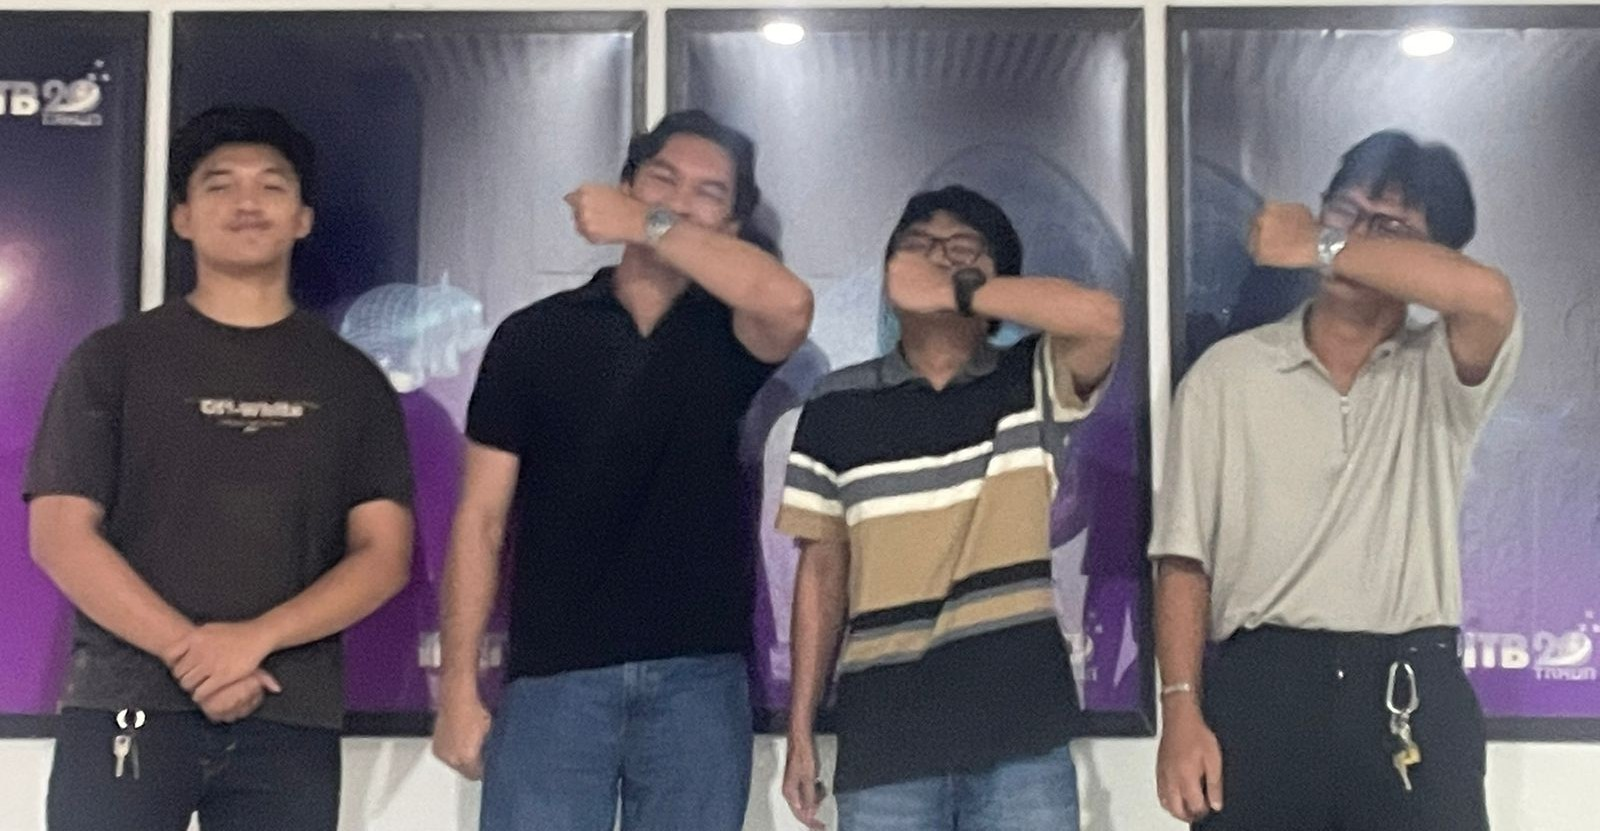
\includegraphics[height=8cm]{nael.jpeg}\\[2cm]

    {\large \textbf{Disusun oleh:}}\\[0.3cm]
    {\large
      \textbf{\GroupName}\\[0.25cm]
      \MemberA\\
      \MemberB\\
      \MemberC\\
      \MemberD\\
    }

    \vfill

    {\large \textsc{\Lab}}\\[0.15cm]
    {\large \textsc{Program Studi \Program}}\\[0.15cm]
    {\large \textsc{\Faculty}}\\[0.15cm]
    {\large \textsc{\University}}\\
  \end{center}
\end{titlepage}

\tableofcontents
\newpage

\section{Pendahuluan}

Bahasa Pemrograman diciptakan sebagai perantara komunikasi antara manusia yang
mengerti logika dan bahasa tingkat tinggi dengan komputer yang hanya dapat
mengerti bahasa mesin (\textit{machine code}). Tanpa adanya bahasa pemrograman,
manusia harus menuliskan instruksi komputer secara tingkat rendah kepada
komputer yang hanya mengerti 0 dan 1. Dalam hierarkinya, bahasa tingkat tinggi
(\textit{high-level}) dirancang agar lebih mendekati bahasa manusia, namun hal ini
menuntut proses transformasi yang berlapis agar dapat dipahami oleh CPU.

\begin{figure}[H]
\centering
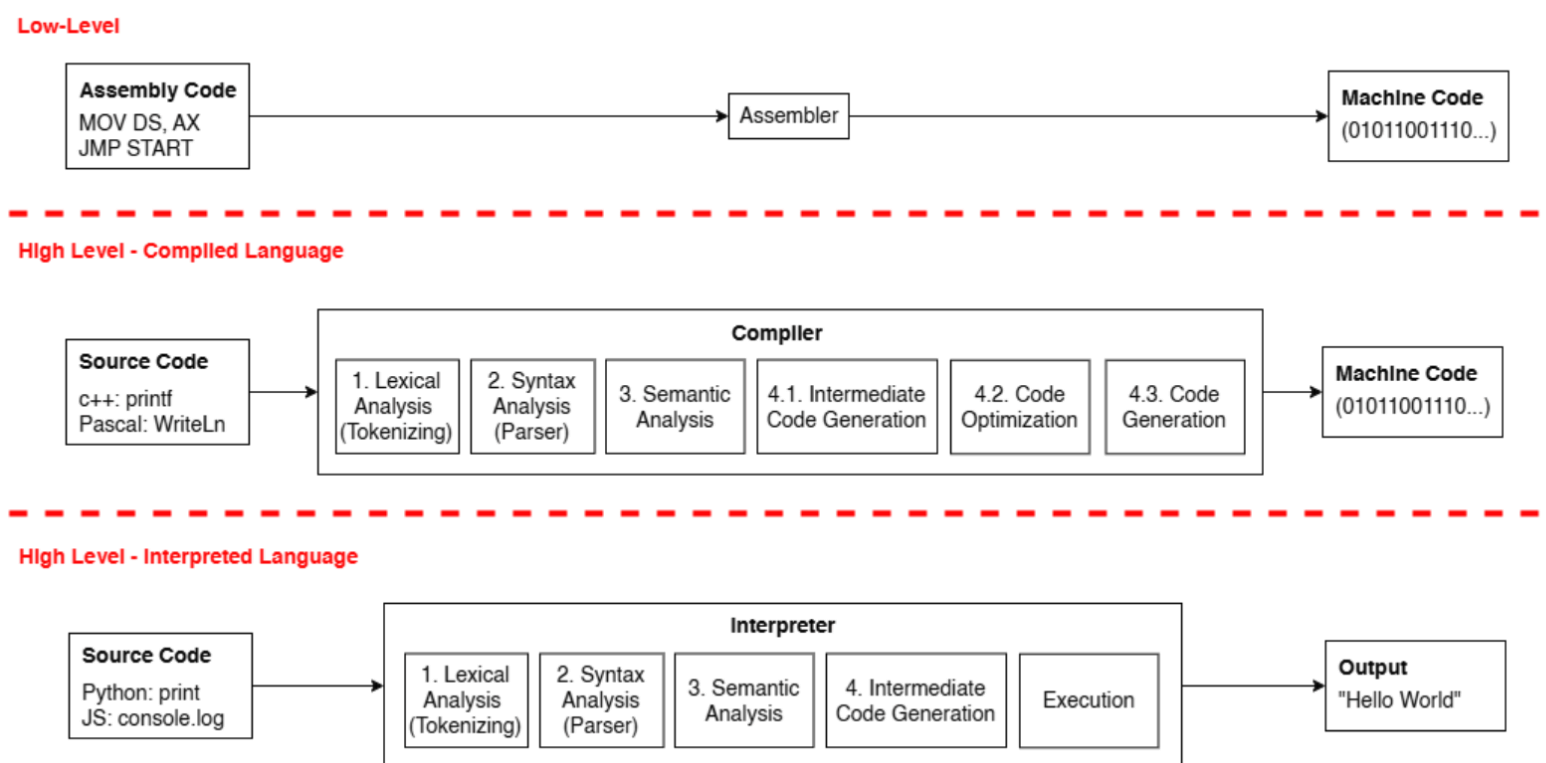
\includegraphics[width=0.8\textwidth]{tipe-bahasa.png}
\caption{Tipe-tipe bahasa pemrograman}
\caption*{Sumber: Asisten IF2224}
\end{figure}

Proses transformasi ini dilakukan melalui mekanisme \textit{compiler} atau
\textit{interpreter}. Tahap awal dan fundamental dalam mekanisme tersebut adalah
Analisis Leksikal (\textit{Lexical Analysis}). Pada tahap ini, kode sumber yang berupa
rangkaian karakter mentah dibaca dan dikelompokkan menjadi satuan makna terkecil
yang disebut token, seperti kata kunci (\textit{keyword}), pengenal
(\textit{identifier}), operator, dan konstanta. Analisis leksikal berperan
krusial dalam menyederhanakan tugas tahap berikutnya, yaitu parsing, dengan
membuang elemen yang tidak relevan seperti spasi dan komentar, serta mendeteksi
simbol invalid sejak awal.

\subsection{Latar Belakang}
Proses kompilasi suatu bahasa pemrograman terdiri atas beberapa tahap yang saling berkaitan, dimulai dari analisis leksikal (\textit{lexical analysis}), analisis sintaktik, analisis semantik, hingga pembangkitan kode (\textit{code generation}). Tahap pertama --- analisis leksikal --- bertanggung jawab untuk membaca kode sumber karakter demi karakter dan mengelompokkannya menjadi satuan-satuan bermakna yang disebut \textit{token}. Keberhasilan tahap ini menjadi fondasi bagi seluruh tahap kompilasi berikutnya.

Pada tugas besar mata kuliah IF2224 Teori Bahasa Formal dan Otomata, mahasiswa diminta untuk membangun sebuah \textit{compiler} sederhana untuk bahasa pemrograman Arion, yaitu bahasa bertipe Pascal. Milestone pertama berfokus pada pembangunan \textit{lexical analyzer} (lexer) yang mampu mengenali seluruh jenis token yang didefinisikan dalam spesifikasi bahasa Arion.

\subsection{Rumusan Masalah}
Bagaimana merancang dan mengimplementasikan sebuah \textit{lexical analyzer} berbasis \textit{Deterministic Finite Automaton} (DFA) yang mampu:
\begin{enumerate}[label=\arabic*.]
  \item Membaca kode sumber bahasa Arion dari berkas masukan.
  \item Mengenali dan mengklasifikasikan setiap leksem ke dalam tipe token yang sesuai (kata kunci, identifier, konstanta, operator, dan komentar).
  \item Menangani kasus-kasus ambigu seperti pembedaan \texttt{charcon} dan \texttt{string}, bilangan bulat dan bilangan riil, serta operator satu dan dua karakter.
  \item Melaporkan kesalahan leksikal dengan informasi nomor baris yang akurat.
\end{enumerate}

\subsection{Gambaran Umum Sistem}
Sistem yang dibangun merupakan sebuah \textit{lexical analyzer} untuk bahasa Arion yang diimplementasikan dalam bahasa C++20. Lexer ini membaca berkas kode sumber, memproses setiap karakter menggunakan logika DFA berbasis \textit{switch-case}, dan menghasilkan daftar token sebagai keluaran. Sistem terdiri atas lima komponen utama: \texttt{SourceBuffer} (pembacaan berkas), \texttt{TokenType} (definisi tipe token), \texttt{Token} (struktur data token), \texttt{Scanner} (mesin DFA), dan \texttt{Logger} (pelaporan kesalahan).

\subsection{Spesifikasi Umum}
\begin{enumerate}[label=\arabic*.]
  \item Mengenali 52 jenis token: 5 tipe literal/nilai (\texttt{intcon}, \texttt{realcon}, \texttt{charcon}, \texttt{string}, \texttt{ident}), 25 kata kunci, 20 operator dan tanda baca, serta \texttt{comment} dan \texttt{eof\_token}.
  \item Kata kunci bersifat \textit{case-insensitive} (\texttt{BEGIN}, \texttt{Begin}, dan \texttt{begin} dikenali sebagai token yang sama).
  \item Mendukung dua gaya komentar: \texttt{\{ \ldots\ \}} dan \texttt{(* \ldots\ *)}.
  \item Melaporkan kesalahan leksikal tanpa menghentikan proses scanning (\textit{error recovery}).
\end{enumerate}


\section{Dasar Teori}

\subsection{Pendefinisian Bahasa Pemrograman}
Bahasa Pemrograman adalah cara manusia untuk dapat memberikan perintah
(\textit{instruction}) kepada sebuah komputer. Setiap bahasa pemrograman
memiliki kata kunci dan aturannya masing-masing serta makna dari kata-kata itu
yang disebut sintaks(\textit{syntax}) dan semantik (\textit{semantics}).
Input yang terdapat kesalahan pada tingkat sintaks berarti input tersebut tidak
valid untuk bahasa pemrograman tersebut, sedangkan kesalahan pada tingkat
semantik umumnya berbentuk kesalahan logika.

\subsubsection{Hierarki Bahasa Pemrograman}
Berdasarkan tingkat abstraksinya, bahasa pemrograman diklasifikasikan menjadi dua kategori utama:
\begin{itemize}
\item \textbf{\textit{Low-Level Language} (Bahasa Tingkat Rendah)}: Bahasa yang instruksinya mendekati arsitektur perangkat keras dan bahasa mesin (biner 0 dan 1). Contohnya adalah \textit{Assembly}, yang memerlukan \textit{Assembler} untuk menerjemahkan kode menjadi instruksi yang dapat dipahami CPU.
\item \textbf{\textit{High-Level Language} (Bahasa Tingkat Tinggi)}: Bahasa yang dirancang agar lebih mudah dibaca dan dipahami oleh manusia karena menggunakan kosakata yang menyerupai bahasa natural. Semakin tinggi tingkat bahasa tersebut, semakin banyak tahapan pemrosesan yang diperlukan untuk mengubahnya menjadi kode mesin. Contoh bahasa tingkat tinggi antara lain Pascal, C++, Python, dan Java.
\end{itemize}

\subsubsection{\textit{Compiler} dan \textit{Interpreter} }
Untuk menjalankan kode sumber yang ditulis dalam bahasa tingkat tinggi,
diperlukan sebuah perangkat lunak penerjemah yang mengubah kode tersebut menjadi
format yang dapat dieksekusi oleh mesin. Secara umum, terdapat dua mekanisme
utama untuk mengubah bahasa tingkat tinggi ke bahasa mesin:

\begin{enumerate}
\item \textbf{\textit{Compiler} (Kompilator)}:
\textit{Compiler} adalah program yang menerjemahkan seluruh \textit{source code}
secara utuh menjadi kode mesin (biasanya dalam bentuk \textit{Object File})
sebelum program dijalankan. Proses kompilasi pada \textit{compiler} umumnya
terdiri dari empat tahapan utama: \textit{Lexical Analysis}, \textit{Syntax
Analysis}, \textit{Semantic Analysis}, dan \textit{Intermediate Code
Generation}. Karakteristik utama \textit{compiler} adalah jika terdeteksi adanya
kesalahan (\textit{error}) di dalam \textit{source code}, maka seluruh proses
kompilasi akan gagal dan program tidak dapat dijalankan.

\item \textbf{\textit{Interpreter}}: 
Berbeda dengan \textit{compiler}, \textit{interpreter} memproses kode sumber
baris demi baris secara langsung. \textit{Interpreter} membaca,
menerjemahkan, dan langsung mengeksekusi kode mesin tersebut baris demi baris.
Hal ini memungkinkan program tetap berjalan normal hingga baris sebelum
ditemukannya kesalahan; misalnya, jika terdapat \textit{error} pada baris ke-10,
baris 1 sampai 9 akan tetap berhasil dieksekusi. Meskipun mekanisme eksekusinya
berbeda, \textit{interpreter} sebenarnya memiliki tahapan pemrosesan internal
yang serupa dengan \textit{compiler}.

\end{enumerate}

\subsection{Teori Kompilator (\textit{Compiler Theory})}

Proses kompilasi adalah urutan dari berbagai fase (\textit{phases}) yang bekerja secara berurutan. Setiap fase mengambil input dari tahap sebelumnya, memprosesnya, dan memberikan output yang akan digunakan sebagai input untuk fase berikutnya. Secara umum, arsitektur sebuah kompilator terdiri dari fase-fase berikut:

\begin{enumerate}
    \item \textbf{\textit{Lexical Analysis}}: Fase pertama yang bekerja sebagai
        pemindai teks (\textit{text scanner}) pada kode sumber. Penjelasan lebih detail mengenai fase ini dibahas pada sub-bab tersendiri di bawah.
    \item \textbf{\textit{Syntax Analysis} (\textit{Parsing})}: Mengambil
        \textit{token} yang dihasilkan oleh \textit{lexical analysis} dan
        membangun pohon sintaksis (\textit{parse tree}). Fase ini memeriksa
        kebenaran susunan \textit{token} berdasarkan aturan tata bahasa
        (\textit{grammar}) kode sumber.
    \item \textbf{\textit{Semantic Analysis}}: Memeriksa apakah pohon sintaksis
        yang dibangun mengikuti aturan semantik bahasa, seperti kecocokan
        operasi tipe data dan memastikan \textit{identifier} telah
        dideklarasikan sebelum digunakan. Fase ini menghasilkan keluaran berupa
        pohon sintaksis yang dianotasi.
    \item \textbf{\textit{Intermediate Code Generation}}: Menghasilkan
        representasi kode perantara untuk mesin abstrak, yang posisinya
        menjembatani antara bahasa tingkat tinggi dan bahasa mesin.
    \item \textbf{\textit{Code Optimization}}: Mengoptimalkan kode perantara
        dengan menghapus baris kode yang tidak perlu dan mengatur ulang urutan
        instruksi. Tujuannya adalah untuk mempercepat eksekusi program tanpa
        membuang sumber daya (\textit{CPU}, memori).
    \item \textbf{\textit{Target Code Generation}}: Merupakan fase sintesis
    akhir (\textit{back-end}) yang menggunakan representasi kode perantara dan
    tabel simbol untuk menghasilkan program target atau bahasa mesin.
\end{enumerate}

\subsubsection{Analisis Leksikal (\textit{Lexical Analysis})}
Sebagai fokus utama pada \textit{milestone} ini, Analisis Leksikal adalah fase
pertama dari sebuah kompilator. Fase ini memproses kode sumber yang ditulis
dalam bentuk kalimat sintaksis dan memecahnya menjadi serangkaian unit bermakna
yang disebut \textit{token}. 

Berdasarkan prinsip desain kompilator, mekanisme kerja dan tugas utama dari
\textit{lexical analyzer} meliputi:
\begin{itemize}
    \item \textbf{Penyaringan Karakter}: \textit{Lexical analyzer} membaca kode
        sumber sebagai aliran karakter (\textit{character stream}) dan secara
        otomatis menghapus seluruh spasi kosong (\textit{whitespace}) maupun
        komentar (\textit{comments}) di dalam kode sumber.
    \item \textbf{Tokenisasi dan Pengenalan \textit{Lexeme}}: Barisan karakter
        (\textit{alphanumeric}) yang memiliki makna diidentifikasi sebagai
        \textit{lexeme}. \textit{Lexeme} ini kemudian dicocokkan dengan aturan
        baku atau pola (\textit{pattern})—yang umumnya didefinisikan melalui
        \textit{regular expression}—untuk divalidasi sebagai sebuah
        \textit{token} (seperti kata kunci, konstanta, \textit{identifier}, atau
        operator).
    \item \textbf{Kerja Sama dengan \textit{Syntax Analyzer} (\textit{Parser})}:
        \textit{Lexical analyzer} bekerja sangat erat dengan \textit{syntax
        analyzer}. Ia memeriksa keberadaan \textit{token} yang legal dan
        meneruskan data \textit{token} tersebut kepada \textit{syntax analyzer}
        hanya pada saat dibutuhkan atau diminta (\textit{when it demands}).
    \item \textbf{Penanganan Kesalahan (\textit{Error Handling})}: Apabila
        \textit{lexical analyzer} memindai urutan karakter yang tidak valid atau
        tidak dapat diklasifikasikan ke dalam pola \textit{token} apa pun, maka
        ia akan langsung menghasilkan pesan kesalahan (\textit{error}).
\end{itemize}

\subsection{Teori Bahasa Formal dan Otomata}

\subsubsection{\textit{Regular Expression}}
\textit{Regular Expression} (RE) adalah sebuah notasi matematis formal yang
digunakan untuk mendeskripsikan suatu bahasa reguler. Dalam kompilator, RE
digunakan secara luas untuk mendefinisikan \textit{pattern} (pola) dari
\textit{token} secara akurat. Dengan menggunakan operasi dasar seperti
\textit{Concatenation} (penyambungan), \textit{Union} (penggabungan alternatif),
dan \textit{Kleene Closure} (perulangan nol kali atau lebih), pembuat bahasa
dapat mendefinisikan aturan rumit, misalnya: "Sebuah identifier harus diawali
dengan huruf, diikuti oleh kombinasi huruf atau angka dengan jumlah berapa pun."

\subsubsection{\textit{Finite Automata} (FA)}

\textit{Finite Automata} (FA) atau \textit{Finite State Machine} (FSM) adalah
model komputasi matematika abstrak yang digunakan untuk mengenali
\textit{Regular Expression}. Dalam konteks kompilator, FA berfungsi sebagai
mesin pemeriksa yang menelusuri karakter masukan untuk memvalidasi apakah urutan
karakter tersebut (\textit{lexeme}) membentuk \textit{token} yang sah sesuai
aturan bahasa.

Secara formal, sebuah \textit{Finite Automata} didefinisikan secara matematis
sebagai \textit{5-tuple} $(Q, \Sigma, \delta, q_0, F)$, yang terdiri dari:
\begin{itemize}
    \item $Q$ : Himpunan hingga dari kedudukan atau \textit{state}.
    \item $\Sigma$ : Himpunan hingga dari simbol \textit{input} atau alfabet
        (contoh: himpunan huruf, angka, dan simbol baca).
    \item $\delta$ : Fungsi transisi yang memetakan $Q \times \Sigma \rightarrow
        Q$ (menentukan \textit{state} tujuan berdasarkan \textit{state} saat ini dan simbol yang dibaca).
    \item $q_0$ : \textit{State} awal (\textit{initial state}), di mana $q_0 \in
        Q$. Mesin selalu memulai komputasi dari \textit{state} ini.
    \item $F$ : Himpunan \textit{state} akhir atau penerima
        (\textit{final/accepting state}), di mana $F \subseteq Q$.
\end{itemize}

Mesin FA membaca masukan berupa \textit{string} karakter demi karakter secara
sekuensial dari kiri ke kanan. Setiap kali membaca satu simbol,
mesin akan berpindah dari \textit{state} saat ini ke \textit{state} berikutnya
sesuai dengan aturan pada fungsi transisi ($\delta$). Jika setelah seluruh
karakter pada masukan selesai dibaca mesin berhenti pada salah satu
\textit{state} yang termasuk dalam himpunan $F$, maka masukan tersebut diterima
(\textit{accepted}) sebagai \textit{token} yang valid. Sebaliknya, jika berhenti
di luar $F$ atau menemukan transisi yang tidak terdefinisi, maka terjadi
\textit{lexical error}.

Berdasarkan sifat penentuan fungsi transisinya, \textit{Finite Automata} dibedakan menjadi dua jenis:
\begin{enumerate}
    \item \textbf{\textit{Nondeterministic Finite Automata} (NFA)}: Suatu mesin
        di mana sebuah \textit{state} dapat memiliki nol, satu, atau lebih jalur
        transisi untuk satu simbol \textit{input} yang sama. NFA juga
        mengizinkan perpindahan \textit{state} tanpa perlu membaca karakter
        \textit{input} (disebut transisi epsilon atau $\epsilon$-transition).
    \item \textbf{\textit{Deterministic Finite Automata} (DFA)}: Suatu mesin di
        mana setiap \textit{state} memiliki tepat satu jalur transisi secara
        mutlak untuk setiap simbol \textit{input} di dalam $\Sigma$. Tidak ada
        ambiguitas jalur dan tidak ada transisi epsilon.
\end{enumerate}

Dalam implementasi program \textit{Lexical Analyzer} yang sebenarnya, model
\textbf{DFA} adalah spesifikasi yang wajib digunakan. Hal ini karena sifat
deterministiknya yang tidak ambigu memungkinkan aturan transisi dikonversi
secara langsung menjadi algoritma terprogram menggunakan pendekatan
\textit{modular} dan penyeleksian kondisi, membaca satu demi satu karakter
hingga menghasilkan klasifikasi \textit{token} yang tepat.

\section{Perancangan \textit{Lexical Analyzer}}

\subsection{Diagram Transisi DFA}

Berikut merupakan rancangan \textit{Deterministic Finite Automata} (DFA) yang dikembangkan untuk mengenali seluruh pembentukan leksikal token pada bahasa pemrograman Arion.

\setlength{\LTleft}{0pt}
\setlength{\LTright}{0pt}
\begin{small}
\setlength{\tabcolsep}{4pt}
\begin{longtable}{|>{\raggedright\arraybackslash}p{2.7cm}|>{\raggedright\arraybackslash}p{2.2cm}|>{\raggedright\arraybackslash}p{2.6cm}|>{\raggedright\arraybackslash}p{2.2cm}|>{\raggedright\arraybackslash}p{5.2cm}|}
\hline
\textbf{Kategori Token} & \textbf{Current State} & \textbf{Input} & \textbf{Next State} & \textbf{Aksi / Keterangan} \\
\hline
\endfirsthead

\hline
\textbf{Kategori Token} & \textbf{Current State} & \textbf{Input} & \textbf{Next State} & \textbf{Aksi / Keterangan} \\
\hline
\endhead

\hline
\multicolumn{5}{r}{\textit{Lanjut ke halaman berikutnya}} \\
\endfoot

\hline
\endlastfoot

\textbf{Identifier \& Keyword} & q0 & [a-zA-Z] & q\_ident & Huruf pertama \\
 & q\_ident & [a-zA-Z0-9] & q\_ident & Loop huruf/angka \\
 & q\_ident & selain itu & accept & Cek keyword / identifier \\
\hline

\textbf{Number} & q0 & [0-9] & q\_number & Angka pertama \\
 & q\_number & [0-9] & q\_number & Loop integer \\
 & q\_number & . & q\_real\_coma & Masuk desimal \\
 & q\_number & selain itu & q\_intcon & Accept integer \\
 & q\_real\_coma & [0-9] & q\_real & Digit setelah titik \\
 & q\_real\_coma & selain itu & q\_error\_1 & Error format real \\
 & q\_real & [0-9] & q\_real & Loop desimal \\
 & q\_real & selain itu & accept & Accept real \\
\hline

\textbf{String \& Char} & q0 & ' & q\_string & Mulai string \\
 & q\_string & selain ' dan EOF & q\_string & Loop isi \\
 & q\_string & ' & accept & Selesai string/char \\
 & q\_string & EOF & q\_error\_2 & Error tidak ditutup \\
\hline

\textbf{Operator Tunggal} & q0 & + & q\_plus & Accept \\
 & q0 & - & q\_minus & Accept \\
 & q0 & * & q\_times & Accept \\
 & q0 & / & q\_rdiv & Accept \\
 & q0 & [ & q\_lbrack & Accept \\
 & q0 & ] & q\_rbrack & Accept \\
 & q0 & , & q\_comma & Accept \\
 & q0 & ; & q\_semicolon & Accept \\
 & q0 & . & q\_period & Accept \\
 & q0 & ) & q\_rparent & Accept \\
\hline

\textbf{Operator Relasional} & q0 & < & q\_< & Kombinasi \\
 & q\_< & = & q\_leq & Accept (<=) \\
 & q\_< & > & q\_neq & Accept (<>) \\
 & q\_< & selain itu & q\_lss & Accept (<) \\
 & q0 & > & q\_> & Kombinasi \\
 & q\_> & = & q\_geq & Accept (>=) \\
 & q\_> & selain itu & q\_gtr & Accept (>) \\
 & q0 & = & q\_= & Kombinasi \\
 & q\_= & = & q\_eql & Accept (==) \\
 & q\_= & selain itu & q\_error\_3 & Error \\
\hline

\textbf{Assignment} & q0 & : & q\_: & Kombinasi \\
 & q\_: & = & q\_becomes & Accept (:=) \\
 & q\_: & selain itu & q\_colon & Accept (:) \\
\hline

\textbf{Komentar (* *)} & q0 & ( & q\_( & Kombinasi \\
 & q\_( & * & q\_comment & Mulai komentar \\
 & q\_comment & selain * & q\_comment & Loop isi \\
 & q\_comment & * ) & accept & Selesai komentar \\
 & q\_comment & EOF & q\_error\_4 & Error tidak ditutup \\
\hline

\textbf{Komentar \{ \}} & q0 & \{ & q\_\{ & Mulai komentar \\
 & q\_\{ & \} & accept & Selesai komentar \\
 & q\_\{ & selain \} & q\_\{ & Loop isi \\
 & q\_\{ & EOF & q\_error\_5 & Error tidak ditutup \\
\hline

\textbf{Whitespace} & q0 & spasi/tab/newline & q0 & Diabaikan \\
\hline

\end{longtable}
\end{small}

\begin{figure}[H]
    \centering
    \includegraphics[width=0.75\textwidth]{dfa1.png} % Pastikan nama file Anda sesuai
    \caption{Diagram Transisi DFA untuk \textit{Lexical Analyzer} Bahasa Arion
    (Part 1)}
    \label{fig:dfa_diagram}
\end{figure}

\begin{figure}[H]
    \centering
    \includegraphics[width=0.75\textwidth]{dfa2.png} % Pastikan nama file Anda sesuai
    \caption{Diagram Transisi DFA untuk \textit{Lexical Analyzer} Bahasa Arion
    (Part 2)}
    \label{fig:dfa_diagram}
\end{figure}

Perancangan diagram transisi DFA ini merupakan representasi logis dari bagaimana \textit{scanner} membaca karakter demi karakter (\textit{character stream}) dan menentukan validitas sebuah \textit{lexeme}. Berdasarkan diagram di atas, terdapat beberapa keputusan desain dan analisis perancangan \textit{state} yang diterapkan:

\subsubsection*{1. Mekanisme \textit{Look-ahead} pada Operator Relasional dan \textit{Assignment}}
Bahasa Arion memiliki operator yang terdiri dari satu karakter (seperti \texttt{+}, \texttt{-}, \texttt{=}) dan multi-karakter (seperti \texttt{<=}, \texttt{>=}, \texttt{<>}, \texttt{:=}). Pada DFA, hal ini ditangani melalui mekanisme \textit{look-ahead}. 
Sebagai contoh, ketika mesin membaca karakter \texttt{<}, ia berpindah ke sebuah \textit{intermediate state}. Dari sana, mesin akan "mengintip" karakter berikutnya:
\begin{itemize}
    \item Jika karakter selanjutnya adalah \texttt{=}, mesin bertransisi ke state akhir untuk token \texttt{leq} (\texttt{<=}).
    \item Jika karakter selanjutnya adalah \texttt{>}, mesin bertransisi ke state akhir untuk token \texttt{neq} (\texttt{<>}).
    \item Jika karakter selanjutnya adalah karakter di luar itu, mesin melakukan \textit{retract} (memundurkan pembacaan) dan menerima input sebagai token \texttt{lss} (\texttt{<}).
\end{itemize}

\subsubsection*{2. Pemisahan State Bilangan Bulat (\texttt{intcon}) dan Riil (\texttt{realcon})}
Penelusuran angka diawali dengan pembacaan digit (\texttt{0-9}). Selama input berupa digit, mesin akan terus berputar pada \textit{state} loop angka tersebut. Untuk mengakomodasi konstanta riil (\texttt{realcon}), DFA menyediakan jalur transisi khusus jika menemukan karakter titik (\texttt{.}). Mesin tidak akan langsung menerima titik tersebut sebagai operator \texttt{period}, melainkan menunggu datangnya digit lanjutan. Jika setelah titik dipastikan terdapat digit tambahan, aliran akan bergeser secara definitif ke rute final \texttt{realcon}. Jika tidak, mesin akan menangani titik tersebut sebagai leksikal terpisah.

\subsubsection*{3. Pengelolaan Literal dan Komentar (\textit{Trap States})}
Literal teks dan karakter dipicu oleh tanda petik tunggal (\texttt{'}). DFA memiliki \textit{state} khusus yang akan terus melahap semua karakter apa pun hingga menemukan tanda petik penutup. Perbedaan validasi panjang untuk \texttt{charcon} (panjang = 1) dan \texttt{string} (panjang $> 1$) didelegasikan pada proses operasional program pasca-DFA.
Selain itu, DFA juga memetakan rute untuk membuang isi komentar. Pembacaan \texttt{\{} atau kombinasi \texttt{(} diikuti \texttt{*} akan membawa mesin ke dalam semacam \textit{trap state} yang terus menerus membaca karakter tanpa membentuk elemen baru, hingga akhirnya menemukan blok penutup \texttt{\}} atau \texttt{*)}.

\subsubsection*{4. Analisis Penggabungan State untuk Token \texttt{ident} dan \textit{Keyword}}
Salah satu keputusan desain yang paling krusial pada DFA ini adalah menyatukan penelusuran \textit{Identifier} (\texttt{ident}) dan seluruh \textit{Keyword} (seperti \texttt{program}, \texttt{var}, \texttt{begin}, dll) ke dalam satu jalur transisi gabungan yang sama (\texttt{q\_ident/keyword}). Keputusan arsitektural ini diambil dengan pertimbangan berikut:
\begin{itemize}
    \item \textbf{Kesamaan Leksikal dan Ekspresi Reguler:} Baik \textit{keyword} maupun \textit{identifier} dibentuk oleh pola ekspresi reguler yang ekuivalen sepenuhnya, yaitu \texttt{[a-z,A-Z][a-z,A-Z,0-9\_]*}. Keduanya wajib diawali oleh alfabet dan bebas diikuti oleh rentetan alfanumerik.
    \item \textbf{Mencegah Fenomena \textit{State Explosion}:} Apabila ke-52 token \textit{keyword} pada spesifikasi Arion dipetakan secara eksplisit huruf demi huruf membentuk sebuah graf berarah (seperti pada struktur data \textit{Trie}), diagram transisi akan menjadi terlampau masif dan tidak proporsional. Hal ini juga memicu kerentanan ambiguitas saat membedakan awalan sebuah variabel (contoh: variabel \texttt{integerKu}) dengan \textit{keyword} yang beririsan (\texttt{integer}).
    \item \textbf{Efisiensi Resolusi Pascakomputasi:} Melalui penggabungan jalur ini, tugas murni mesin DFA disederhanakan hanya untuk mengekstrak satu rentetan kata yang valid secara leksikal. Setelah *accepting state* tercapai, proses validasi dilimpahkan pada kode program. Algoritma akan melakukan pencarian (\textit{lookup}) nilai \textit{lexeme} tersebut pada Tabel \textit{Keyword} terpusat (\textit{Hash Map}). Jika ditemukan kesamaan, maka token secara spesifik diklasifikasikan sebagai \textit{keyword} (misal: \texttt{varsy}). Sebaliknya jika hasil nihil, secara *default* token tersebut diresmikan sebagai \texttt{ident} reguler.
\end{itemize}

\subsection{Struktur Program \textit{Lexical Analyzer}}

Tahapan pertama dalam \textit{compiler} ini adalah \textit{Lexical Analyzer} (Scanner) yang bertugas membaca \textit{source code} karakter demi karakter dari \texttt{SourceBuffer} dan mengelompokkannya menjadi \textit{Token}. Implementasi pada \texttt{Scanner.cpp} dan \texttt{Scanner.hpp} dibangun dengan secara langsung mereplikasi logika kerja \textit{Deterministic Finite Automaton} (DFA) yang telah dijabarkan sebelumnya.

\subsubsection{Struktur Proyek}

Struktur implementasi untuk \textit{lexical analyzer} pada proyek ini berfokus pada folder \texttt{src/lexical} dengan pembagian berkas sebagai berikut:
\begin{itemize}
  \item \texttt{SourceBuffer.hpp} \& \texttt{.cpp}: modul pembaca berkas sumber yang menyediakan akses karakter per karakter secara aman, termasuk operasi utilitas \textit{look-ahead}.
  \item \texttt{Scanner.hpp} \& \texttt{.cpp}: deklarasi dan implementasi kelas \texttt{Scanner} yang menjadi jantung dari mesin \textit{lexical analyzer}.
  \item \texttt{Token.hpp}: representasi unit objek token beserta atribut esensialnya (jenis terminal, nilai \textit{lexeme}, dan metadata penunjuk baris).
  \item \texttt{TokenType.hpp}: definisi enumerasi dari seluruh simpul terminal (52 tipe token) yang dikenali dan dipersyaratkan oleh spesifikasi bahasa Arion.
  \item \texttt{Logger.hpp}: utilitas sistem pelaporan untuk memunculkan pesan peringatan diagnostik selama tahap kompilasi (*lexical errors*).
\end{itemize}

\subsubsection{Klasifikasi Implementasi Alur DFA dalam Program}

Siklus mesin direpresentasikan oleh perulangan \texttt{scanToken()}. Saat fungsi ini dipanggil, ia bertindak seolah-olah mesin me-reset kembali ke \textit{Start State} ($q_0$). Percabangan logika implementasi didasarkan pada pembacaan karakter awal \texttt{advance()} dengan *switch-case* atau percabangan if, membentuk modul sebagai berikut:

\begin{itemize}
    \item \textbf{Modul 1: Identifier \& Keywords (\texttt{q\_ident/keyword})}\\
    Jika evaluasi mengembalikan fungsi valid \texttt{isAlpha()}, siklus memanggil \texttt{Scanner::identifier()}. Dalam metode ini, program membaca karakter selanjutnya (\textit{looping}) secara kontinu selama fungsi \texttt{isAlphaNumeric()} masih bernilai *true*. Saat bertemu karakter asing, iterasi diputus. Teks \textit{lexeme} yang terakumulasi lantas diekstrak dan dicocokkan dengan kontainer tabel konstanta \textit{keyword} (\texttt{unordered\_map}). Kecocokan berbuah \textit{Token Keyword} (\texttt{programsy}, \texttt{forsy}, dll); jika tidak, instansiasi mengembalikan \textit{Token} \texttt{ident}.

    \item \textbf{Modul 2: Numbers - intcon \& realcon (\texttt{q\_number\_int, q\_real\_number})}\\
    Menemukan awalan digit angka mendelegasikan alur ke \texttt{Scanner::number()}. Blok perulangan primitif mengekstrak deret murni bilangan bulat. Melalui pendekatan *look-ahead*, mesin kemudian menguji validitas karakter titik `\texttt{.}' di depannya. Konformitas \textit{match} (titik diikuti digit) memicu program mengakumulasi komposit tipe nilai primitif bilangan riil (berujung \textit{Token} \texttt{realcon}). Tanpa validasi tersebut, nilai default yang diteruskan secara presisi adalah \textit{Token} \texttt{intcon}.

    \item \textbf{Modul 3: Strings \& Chars (\texttt{q\_string\_char})}\\
    Pemicu petik tunggal `\texttt{'}' melompat ke rutinitas \texttt{Scanner::stringLiteral()}. Secara sederhana program mengolah teks bebas di dalamnya hingga blok penutup kutip terkalibrasi. Selesai memindai, evaluasi dihitung: panjang tepat 1 karakter menyuntikkan kategori \texttt{charcon}, sedangkan lebih dari itu bermuara sebagai \texttt{string}. Modul ini dibekali dengan interupsi \textit{error handling} seandainya baris berakhir gantung (*Unterminated string*).

    \item \textbf{Modul 4: Operators \& Delimiters}\\
    Karakter tunggal terminal absolut (spt: \texttt{+}, \texttt{*}, \texttt{;}, \texttt{,}) memiliki *node accepting state* permanen dan langsung diregister menjadi simbol terminal. Tipe multi-operator memanfaatkan delegasi pergeseran via fungsi \texttt{match()}:
    \begin{itemize}
        \item Simbol \texttt{:} akan menguji metode \texttt{match('=')}. Retur presisi mencetak \texttt{becomes} (\texttt{:=}). Ketiadaan retur berbuah terminal tunggal \texttt{colon} (\texttt{:}).
        \item Skema ekuivalen membentengi karakter \texttt{<} yang sanggup bercabang ke \texttt{leq} (\texttt{<=}), \texttt{neq} (\texttt{<>}), hingga *fallback* tunggal \texttt{lss} (\texttt{<}). Serta pada \texttt{>} yang mencakup \texttt{geq} (\texttt{>=}) atau \texttt{gtr} (\texttt{>}).
    \end{itemize}

    \item \textbf{Modul 5: Penanganan Whitespace \& Comments}\\
    \textit{Whitespace} murni layaknya spasi, tabulasi (\texttt{\char`\\t}), dan \textit{carriage return} (\texttt{\char`\\r}) secara utuh digugurkan eksistensinya tanpa mencetak token (lompatan balik siklik pada DFA). Transisi *newline* (\texttt{\char`\\n}) dimanfaatkan pasif sebagai *tracker* eskalasi baris.
    Di ranah *comments*, insiden identifikasi pembuka blok (spt \texttt{\{} atau \texttt{(*} ) mengaktivasikan pengurasan karakter \textit{dummy loop} (*trap state*) ke dalam *buffer* kosong hingga mendeteksi entitas kutub pasangannya masing-masing.
\end{itemize}

Seluruh mekanisme program berpedoman pada manuver pergeseran \textit{pointer} alami yang mencerminkan topologi transisi diagram. Kompilasi unit valid tersebut akan diteruskan secara konsisten menuju inisialisasi pada \textit{constructor} statis dari kelas \texttt{Token}.

\subsection{Token: Tipe dan Nilai}
Sebuah \textit{token} terdiri atas dua komponen utama: \textbf{tipe token} (\textit{token type}) yang menunjukkan kategori leksikal, dan \textbf{nilai} (\textit{value/lexeme}) yang menyimpan representasi teks aslinya. Sebagai contoh dalam bahasa Arion:

\begin{table}[H]
  \centering
  \begin{tabular}{llp{6cm}}
    \toprule
    \textbf{Leksem} & \textbf{Tipe Token} & \textbf{Keterangan} \\
    \midrule
    \texttt{program}  & \texttt{programsy} & Kata kunci deklarasi program \\
    \texttt{myVar}    & \texttt{ident}     & Identifier yang didefinisikan pengguna \\
    \texttt{42}       & \texttt{intcon}    & Konstanta bilangan bulat \\
    \texttt{3.14}     & \texttt{realcon}   & Konstanta bilangan riil \\
    \texttt{'a'}      & \texttt{charcon}   & Konstanta karakter tunggal \\
    \texttt{'hello'}  & \texttt{string}    & Literal string (lebih dari satu karakter) \\
    \texttt{:=}       & \texttt{becomes}   & Operator penugasan \\
    \texttt{==}       & \texttt{eql}       & Operator persamaan \\
    \bottomrule
  \end{tabular}
  \caption{Contoh token dalam bahasa Arion}
\end{table}

Bahasa Arion mendefinisikan total 52 jenis token yang mencakup literal, kata kunci, operator aritmetika, operator logika, operator perbandingan, tanda baca, serta token khusus untuk komentar dan akhir berkas.

\subsection{Hubungan Bahasa Reguler dan Pola Token}
Setiap jenis token dalam suatu bahasa pemrograman dapat dideskripsikan oleh sebuah ekspresi reguler (\textit{regular expression}). Sebagai contoh:
\begin{itemize}[leftmargin=1.5em]
  \item \textbf{Identifier:} \verb|[a-zA-Z_][a-zA-Z0-9_]*| --- dimulai oleh huruf atau \textit{underscore}, diikuti oleh nol atau lebih karakter alfanumerik.
  \item \textbf{Integer:} \verb|[0-9]+| --- satu atau lebih digit.
  \item \textbf{Real:} \verb|[0-9]+\.[0-9]+| --- digit, titik, lalu digit lagi.
  \item \textbf{Operator dua karakter:} \verb|:=|, \verb|==|, \verb|<=|, \verb|>=|, \verb|<>| --- urutan dua karakter tetap.
\end{itemize}

Berdasarkan teorema Kleene, setiap bahasa yang dapat dideskripsikan oleh ekspresi reguler merupakan bahasa reguler dan dapat dikenali oleh DFA. Oleh karena itu, pendekatan berbasis DFA memberikan jaminan teoritis bahwa semua pola token dapat dikenali secara efisien dan deterministik.

% ============================================================
%   SECTION 3 — PERANCANGAN DAN IMPLEMENTASI
% ============================================================

\section{Implementasi}

\subsection{Pendekatan Modular pada DFA}
DFA lexer Arion dirancang dengan pendekatan \textit{modular}: state awal $q_0$ berfungsi sebagai \textit{dispatcher} yang memeriksa karakter pertama dan mendelegasikan pemrosesan ke modul-modul khusus. Pendekatan ini dipilih karena:
\begin{enumerate}[label=\arabic*.]
  \item Setiap modul menangani satu kategori token sehingga kompleksitas logika terisolasi.
  \item Penambahan pola token baru cukup dilakukan pada modul yang relevan tanpa mengubah modul lain.
  \item Memudahkan pengujian dan \textit{debugging} per modul secara independen.
\end{enumerate}

Berikut adalah modul-modul utama dalam DFA:

\subsubsection{Modul Identifier dan Kata Kunci (\textit{q\_identifyModule})}
Modul ini dimasuki ketika karakter pertama adalah huruf atau \textit{underscore}. Scanner terus membaca karakter alfanumerik hingga menemukan karakter non-alfanumerik, lalu melakukan \textit{retract} (tidak mengonsumsi karakter terakhir). Leksem yang terkumpul dikonversi ke huruf kecil dan dicari dalam tabel kata kunci. Jika ditemukan, token kata kunci yang sesuai dihasilkan; jika tidak, token \texttt{ident} dihasilkan dengan leksem asli (mempertahankan huruf besar/kecil asli).

\begin{lstlisting}[style=cpp, caption={Penanganan identifier dan kata kunci}]
void Scanner::identifier() {
    while (isAlphaNumeric(peek()))
        advance();
    string text = source.substring(start, current - start);
    string lower = toLower(text);
    auto it = keywords.find(lower);
    if (it != keywords.end())
        addToken(it->second);
    else
        addToken(TokenType::ident, Literal{text});
}
\end{lstlisting}

\subsubsection{Modul Bilangan (\textit{q\_number\_module})}
Modul ini dimasuki ketika karakter pertama adalah digit. Scanner membaca digit berturut-turut. Jika setelah titik (\texttt{.}) terdapat digit lagi, maka bilangan diklasifikasikan sebagai \texttt{realcon}; jika tidak, bilangan menjadi \texttt{intcon} dan titik diperlakukan sebagai token \texttt{period} terpisah.

\begin{lstlisting}[style=cpp, caption={Penanganan bilangan bulat dan riil}]
void Scanner::number() {
    while (isdigit(static_cast<unsigned char>(peek())))
        advance();
    if (peek() == '.' &&
        isdigit(static_cast<unsigned char>(peekNext()))) {
        advance(); // konsumsi '.'
        while (isdigit(static_cast<unsigned char>(peek())))
            advance();
        addToken(TokenType::realcon, /* nilai double */);
    } else {
        addToken(TokenType::intcon, /* nilai integer */);
    }
}
\end{lstlisting}

\subsubsection{Modul String dan Charcon}
Modul ini dimasuki ketika karakter \texttt{'} (kutip tunggal) ditemukan. Scanner membaca karakter hingga menemukan kutip penutup. Setelah isi literal diekstrak, panjangnya diperiksa: jika tepat satu karakter, token \texttt{charcon} dihasilkan; jika lebih (atau nol), token \texttt{string} dihasilkan. Jika kutip penutup tidak ditemukan hingga akhir berkas, kesalahan dilaporkan.

\subsubsection{Modul Komentar}
Dua gaya komentar didukung: komentar kurung kurawal \texttt{\{ \ldots\ \}} dan komentar parenthesis-bintang \texttt{(* \ldots\ *)}. Pada kedua kasus, seluruh isi komentar dikonsumsi tanpa menghasilkan token apa pun. Komentar \textbf{tidak bersarang}: pada gaya \texttt{\{ \}}, karakter \texttt{\{} di dalam komentar diabaikan dan komentar ditutup oleh \texttt{\}} pertama yang ditemui.

\subsubsection{Modul Operator Dua Karakter}
Untuk operator yang terdiri atas dua karakter (\texttt{:=}, \texttt{==}, \texttt{<=}, \texttt{>=}, \texttt{<>}), scanner menggunakan metode \texttt{match()} sebagai \textit{lookahead}. Setelah membaca karakter pertama, \texttt{match()} memeriksa apakah karakter berikutnya melengkapi operator dua karakter. Jika ya, kedua karakter dikonsumsi; jika tidak, hanya karakter pertama yang menjadi token.

\begin{lstlisting}[style=cpp, caption={Contoh lookahead untuk operator :=}]
case ':':
    if (match('='))
        addToken(TokenType::becomes);  // :=
    else
        addToken(TokenType::colon);    // :
    return;
\end{lstlisting}

\subsection{Mekanisme \textit{Retract} dan \textit{Lookahead}}
Scanner menggunakan dua pointer: \texttt{start} (awal leksem saat ini) dan \texttt{current} (posisi baca saat ini). Metode \texttt{advance()} mengonsumsi satu karakter dan memajukan \texttt{current}, sedangkan \texttt{peek()} dan \texttt{peekNext()} membaca karakter berikutnya \textbf{tanpa} memajukan pointer. Pola ini memungkinkan scanner melakukan keputusan secara deterministik tanpa perlu \textit{backtracking} yang mahal.

\subsection{Penanganan \textit{Case-Insensitivity}}
Kata kunci dalam bahasa Arion bersifat \textit{case-insensitive}. Implementasinya dilakukan dengan mengonversi leksem ke huruf kecil menggunakan \texttt{toLower()} sebelum pencarian di tabel kata kunci (\texttt{unordered\_map}). Leksem asli tetap disimpan untuk keperluan pelaporan dan modul-modul berikutnya.

\subsection{Struktur Kelas dan Tanggung Jawab}

\begin{table}[H]
  \centering
  \begin{tabular}{lp{9cm}}
    \toprule
    \textbf{Kelas/Berkas} & \textbf{Tanggung Jawab} \\
    \midrule
    \texttt{SourceBuffer} & Membaca berkas kode sumber ke dalam buffer string. Menyediakan akses karakter per posisi (\texttt{at()}) dan ekstraksi substring (\texttt{substring()}). Mengisolasi operasi I/O dari logika DFA. \\
    \texttt{TokenType} & Mendefinisikan \texttt{enum class TokenType} dengan 52 anggota dan fungsi \texttt{tokenTypeName()} untuk konversi ke string. \\
    \texttt{Token} & Struktur data yang menyimpan tipe token, leksem, literal (berupa \texttt{variant<monostate, string, double>}), dan nomor baris. Menyediakan fungsi \texttt{printToken()} untuk keluaran format standar. \\
    \texttt{Scanner} & Mesin utama DFA. Mengelola pointer \texttt{start}/\texttt{current}, mengimplementasikan \texttt{scanToken()} dengan \textit{switch-case}, serta mendelegasikan ke metode-metode modul. \\
    \texttt{Logger} & Melaporkan kesalahan leksikal ke \texttt{stderr} dengan format \texttt{[line N] Error: pesan}. \\
    \texttt{main.cpp} & Titik masuk program. Membaca nama berkas dari argumen, membuat objek \texttt{Scanner}, dan memanggil \texttt{printAllTokens()}. \\
    \bottomrule
  \end{tabular}
  \caption{Pembagian tanggung jawab kelas}
\end{table}

\subsection{Struktur Direktori Proyek}
\begin{lstlisting}[style=bash, caption={Tata letak direktori proyek}]
HBB-Tubes-IF2224-2026/
    src/
        main.cpp                # Titik masuk program
        lexical/
            SourceBuffer.hpp/cpp  # Pembacaan berkas
            TokenType.hpp         # Definisi tipe token
            Token.hpp/cpp         # Struktur dan pencetakan token
            Scanner.hpp/cpp       # Mesin DFA utama
            Logger.hpp            # Pelaporan kesalahan
    test/
        input/                  # Berkas-berkas uji masukan
    doc/                        # Laporan dan dokumentasi
    Makefile                    # Skrip kompilasi
\end{lstlisting}

Arsitektur modular yang digunakan pada lexer dirancang untuk memudahkan pengembangan pada milestone berikutnya. Daftar token yang dihasilkan oleh \texttt{Scanner} dapat langsung dikonsumsi oleh \textit{parser} (analisis sintaktik) tanpa modifikasi antarmuka. Struktur \texttt{Token} yang menyimpan informasi nomor baris memungkinkan pelaporan kesalahan yang akurat pada tahap analisis semantik. Selain itu, pemisahan \texttt{SourceBuffer} dari \texttt{Scanner} memungkinkan penggantian sumber masukan (misalnya dari string langsung untuk pengujian unit) tanpa mengubah logika DFA.

% ============================================================
%   SECTION 4 — PENGUJIAN
% ============================================================

\section{Pengujian}

Pengujian dilakukan terhadap berbagai kasus masukan untuk memverifikasi kebenaran lexer. Setiap kasus uji dijalankan dengan perintah \texttt{make run FILE=<nama\_berkas>}. Keluaran pada \texttt{stdout} (daftar token) dan \texttt{stderr} (pesan kesalahan) dibandingkan dengan hasil yang diharapkan.

\subsection{Kasus Uji 1: Kata Kunci dalam Berbagai Huruf Besar/Kecil}
\textbf{Berkas:} \texttt{edge\_keywords\_case.txt}

\textbf{Masukan:}
\begin{lstlisting}[style=default]
BEGIN While PROGRAM
End If THEN
REPEAT downto NOT
DIV Mod Or
\end{lstlisting}

\textbf{Keluaran yang diharapkan:} \texttt{beginsy}, \texttt{whilesy}, \texttt{programsy}, \texttt{endsy}, \texttt{ifsy}, \texttt{thensy}, \texttt{repeatsy}, \texttt{downtosy}, \texttt{notsy}, \texttt{idiv}, \texttt{imod}, \texttt{orsy} --- total 12 token kata kunci.

\begin{figure}[H]
  \centering
  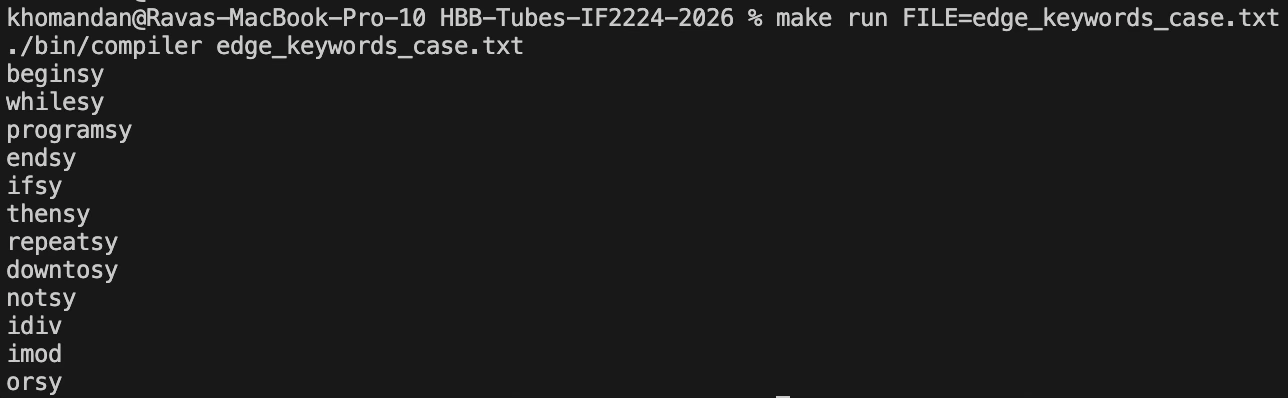
\includegraphics[width=0.7\textwidth]{testcase1.png}
  \caption{Hasil pengujian kasus uji 1}
\end{figure}

\textbf{Analisis:} Seluruh kata kunci dikenali dengan benar meskipun ditulis dengan variasi huruf besar/kecil, membuktikan bahwa mekanisme \texttt{toLower()} bekerja sesuai spesifikasi.

\subsection{Kasus Uji 2: Ambiguitas Bilangan Riil vs Titik}
\textbf{Berkas:} \texttt{edge\_real\_vs\_period.txt}

\textbf{Masukan:}
\begin{lstlisting}[style=default]
end.
3.14
42.
100.0
5 .3
\end{lstlisting}

\textbf{Keluaran yang diharapkan:} \texttt{endsy}, \texttt{period}, \texttt{realcon (3.14)}, \texttt{intcon (42)}, \texttt{period}, \texttt{realcon (100)}, \texttt{intcon (5)}, \texttt{period}, \texttt{intcon (3)} --- total 9 token.

\begin{figure}[H]
  \centering
  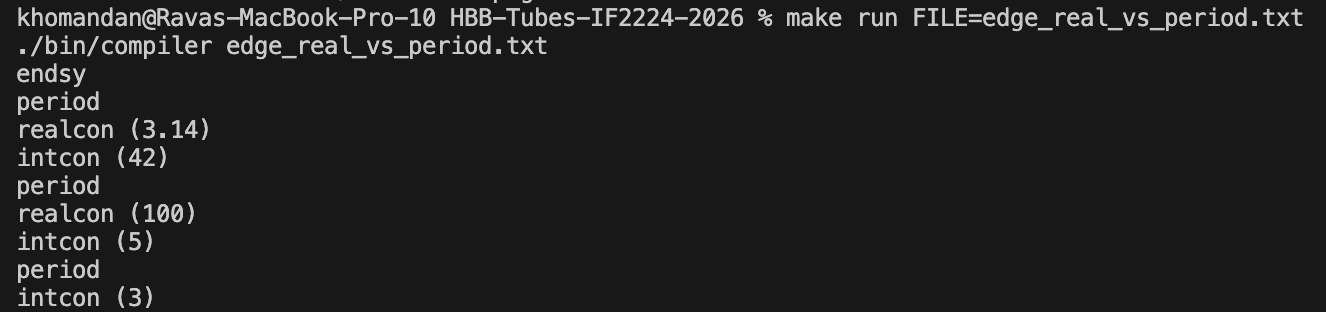
\includegraphics[width=0.7\textwidth]{testcase2.png}
  \caption{Hasil pengujian kasus uji 2}
\end{figure}

\textbf{Analisis:} Scanner membedakan \texttt{realcon} dan \texttt{period} berdasarkan \textit{lookahead}: titik hanya menjadi bagian bilangan riil jika diikuti digit. Kasus \texttt{42.} menghasilkan \texttt{intcon} + \texttt{period} karena tidak ada digit setelah titik.

\subsection{Kasus Uji 3: Charcon vs String}
\textbf{Berkas:} \texttt{edge\_charcon\_vs\_string.txt}

\textbf{Masukan:}
\begin{lstlisting}[style=default]
'a'
'ab'
'hello world'
'x'
''
\end{lstlisting}

\textbf{Keluaran yang diharapkan:} \texttt{charcon (a)}, \texttt{string (ab)}, \texttt{string (hello world)}, \texttt{charcon (x)}, \texttt{string ()} --- total 5 token.

\begin{figure}[H]
  \centering
  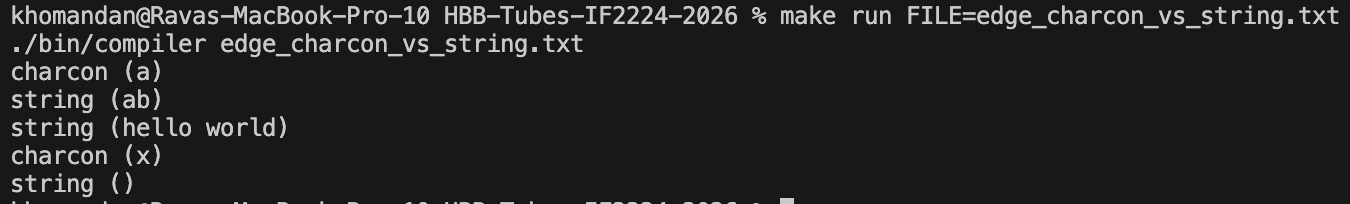
\includegraphics[width=0.7\textwidth]{testcase3.png}
  \caption{Hasil pengujian kasus uji 3}
\end{figure}

\textbf{Analisis:} Literal dengan tepat satu karakter menjadi \texttt{charcon}; selainnya (termasuk literal kosong \texttt{''}) menjadi \texttt{string}. Perilaku ini sesuai dengan logika \texttt{val.length() == 1} pada \texttt{stringLiteral()}.

\subsection{Kasus Uji 4: Komentar Bersarang dan Berkas Hanya Komentar}
\textbf{Berkas:} \texttt{edge\_nested\_comment.txt} dan \texttt{edge\_only\_comments.txt}

\textbf{Masukan (komentar bersarang):}
\begin{lstlisting}[style=default]
{ comment with { nested brace }
x
\end{lstlisting}

\textbf{Keluaran yang diharapkan:} \texttt{ident (x)} --- komentar dikonsumsi seluruhnya, hanya \texttt{x} yang tersisa.

\textbf{Masukan (hanya komentar):} Berkas yang hanya berisi komentar \texttt{\{\}} dan \texttt{(* *)}.

\textbf{Keluaran yang diharapkan:} Tidak ada token yang dicetak.

\begin{figure}[H]
  \centering
  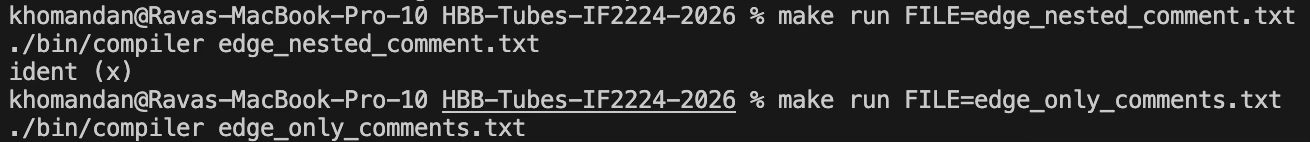
\includegraphics[width=0.7\textwidth]{testcase4.png}
  \caption{Hasil pengujian kasus uji 4}
\end{figure}

\textbf{Analisis:} Komentar tidak bersarang; kurung kurawal \texttt{\{} di dalam komentar diabaikan. Berkas yang hanya mengandung komentar menghasilkan keluaran kosong, membuktikan bahwa komentar tidak menghasilkan token.

\subsection{Kasus Uji 5: Konstruksi yang Tidak Ditutup}
\textbf{Berkas:} \texttt{edge\_unterminated.txt} dan \texttt{edge\_unterminated\_comment.txt}

\textbf{Masukan:} String literal tanpa kutip penutup (\texttt{'hello}) dan komentar tanpa kurung penutup (\texttt{\{ never ends}).

\textbf{Keluaran yang diharapkan (stderr):}
\begin{lstlisting}[style=default]
[line 2] Error: Unterminated string or character literal.
[line 2] Error: Unterminated comment.
\end{lstlisting}

\begin{figure}[H]
  \centering
  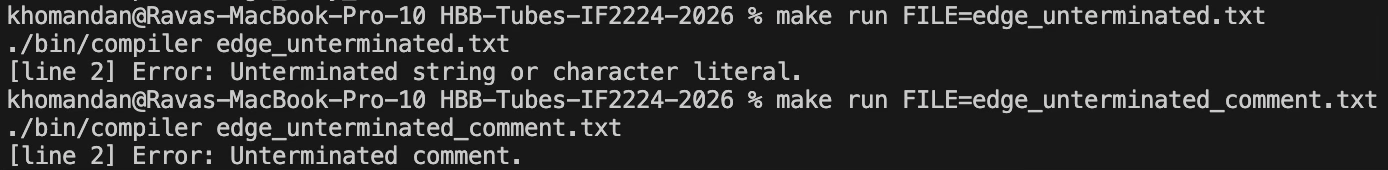
\includegraphics[width=0.7\textwidth]{testcase5.png}
  \caption{Hasil pengujian kasus uji 5}
\end{figure}

\textbf{Analisis:} Lexer melaporkan kesalahan dengan nomor baris yang akurat dan tidak mengalami \textit{crash}. Scanner meneruskan pemrosesan setelah menemukan kesalahan (\textit{error recovery}).

\subsection{Kasus Uji 6: Operator \texttt{==} vs Karakter \texttt{=} Tunggal}
\textbf{Berkas:} \texttt{edge\_eql\_vs\_single\_eq.txt}

\textbf{Masukan:}
\begin{lstlisting}[style=default]
x == 5
y = 3
== ==
\end{lstlisting}

\textbf{Keluaran yang diharapkan (stdout):} \texttt{ident (x)}, \texttt{eql}, \texttt{intcon (5)}, \texttt{ident (y)}, \texttt{intcon (3)}, \texttt{eql}, \texttt{eql}.

\textbf{Keluaran yang diharapkan (stderr):} \texttt{[line 2] Error: Unexpected character: =}

\begin{figure}[H]
  \centering
  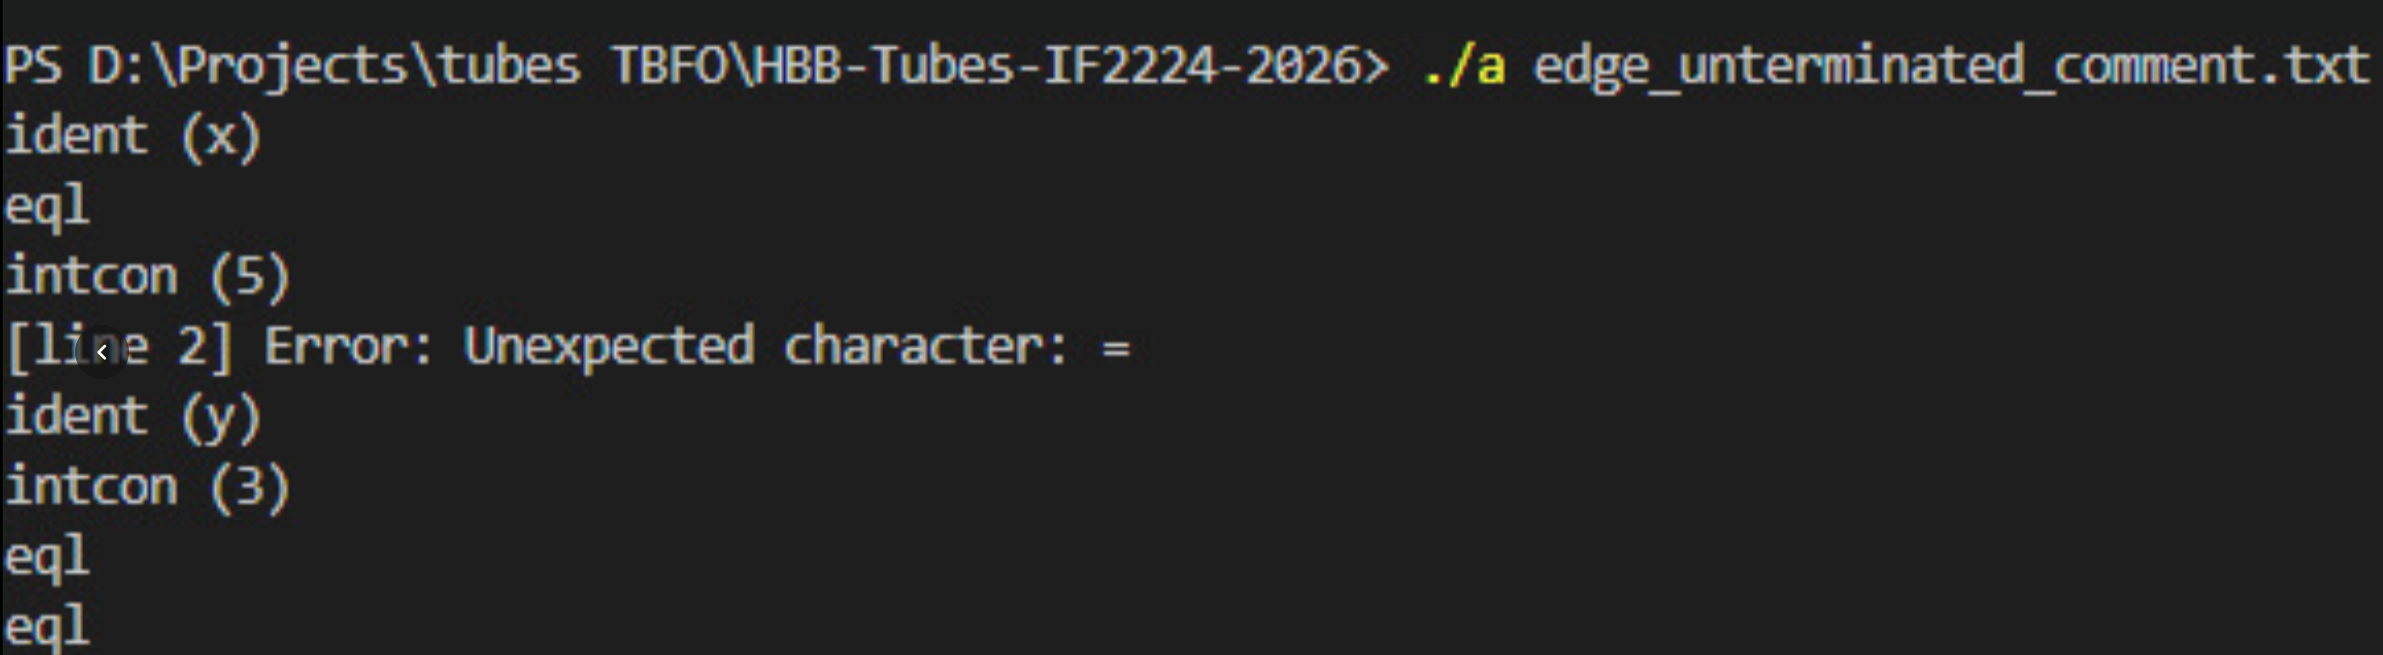
\includegraphics[width=0.7\textwidth]{testcase6.png}
  \caption{Hasil pengujian kasus uji 6}
\end{figure}

\textbf{Analisis:} Operator \texttt{==} dikenali sebagai \texttt{eql}, sedangkan karakter \texttt{=} tunggal (tanpa diikuti \texttt{=}) menghasilkan kesalahan karena bukan operator valid dalam Arion.

\subsection{Kasus Uji 7: Operator \texttt{:=} vs \texttt{:} Diikuti Karakter Lain}
\textbf{Berkas:} \texttt{edge\_becomes\_vs\_colon.txt}

\textbf{Masukan:}
\begin{lstlisting}[style=default]
x := 10
y : integer
a :=b
c: d
\end{lstlisting}

\textbf{Keluaran yang diharapkan:} \texttt{ident (x)}, \texttt{becomes}, \texttt{intcon (10)}, \texttt{ident (y)}, \texttt{colon}, \texttt{ident (integer)}, \texttt{ident (a)}, \texttt{becomes}, \texttt{ident (b)}, \texttt{ident (c)}, \texttt{colon}, \texttt{ident (d)} --- total 12 token.

\begin{figure}[H]
  \centering
  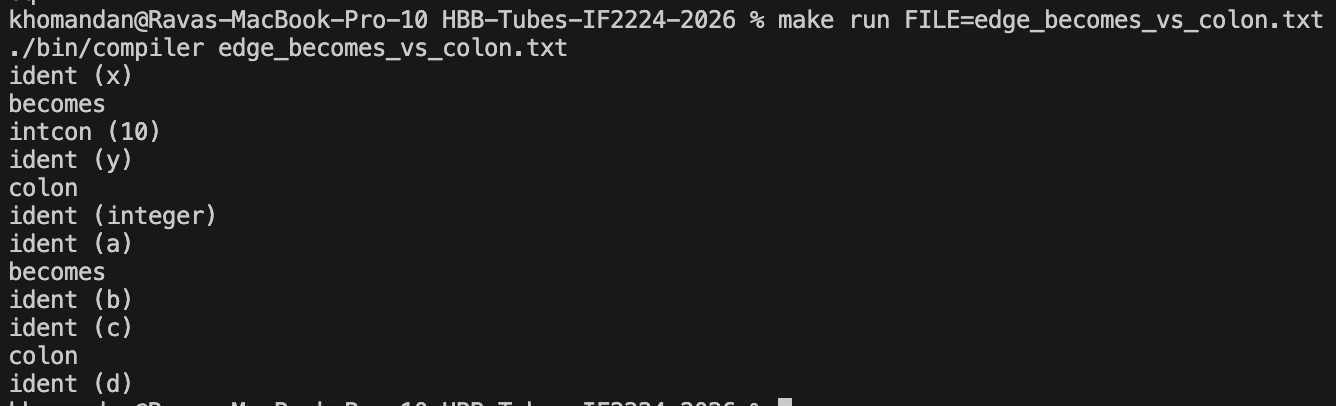
\includegraphics[width=0.7\textwidth]{testcase7.png}
  \caption{Hasil pengujian kasus uji 7}
\end{figure}

\textbf{Analisis:} Mekanisme \texttt{match('=')} berhasil membedakan \texttt{:=} (becomes) dari \texttt{:} (colon). Perhatikan bahwa \texttt{integer} bukan kata kunci dalam Arion sehingga dikenali sebagai \texttt{ident}.

\subsection{Ringkasan Hasil Pengujian}

\begin{table}[H]
  \centering
  \begin{tabular}{clcc}
    \toprule
    \textbf{No.} & \textbf{Deskripsi Kasus Uji} & \textbf{Status} & \textbf{Kesalahan} \\
    \midrule
    1 & Kata kunci berbagai \textit{case}  & Lulus & Tidak ada \\
    2 & Bilangan riil vs titik             & Lulus & Tidak ada \\
    3 & Charcon vs string                  & Lulus & Tidak ada \\
    4 & Komentar bersarang \& hanya komentar & Lulus & Tidak ada \\
    5 & Konstruksi tidak ditutup            & Lulus & 2 kesalahan (sesuai harapan) \\
    6 & \texttt{==} vs \texttt{=} tunggal   & Lulus & 1 kesalahan (sesuai harapan) \\
    7 & \texttt{:=} vs \texttt{:}           & Lulus & Tidak ada \\
    \bottomrule
  \end{tabular}
  \caption{Ringkasan hasil pengujian}
\end{table}

Seluruh kasus uji menghasilkan keluaran yang sesuai dengan ekspektasi. Pesan kesalahan pada kasus uji 5 dan 6 muncul pada \texttt{stderr} dengan nomor baris yang tepat.

\section{Akhiran}

\subsection{Kesimpulan}
Pada milestone pertama ini, kelompok berhasil merancang dan mengimplementasikan \textit{lexical analyzer} untuk bahasa Arion dengan hasil sebagai berikut:
\begin{enumerate}[label=\arabic*., leftmargin=2em]
  \item \textbf{DFA berbasis modul} --- Lexer berhasil mengimplementasikan DFA dengan pendekatan modular yang memisahkan pengenalan identifier, bilangan, string, komentar, dan operator ke dalam modul-modul independen. Seluruh 52 jenis token dapat dikenali dengan benar.
  \item \textbf{Penanganan ambiguitas} --- Kasus-kasus ambigu seperti pembedaan \texttt{charcon} vs \texttt{string} (berdasarkan panjang), \texttt{intcon} vs \texttt{realcon} (berdasarkan \textit{lookahead} setelah titik), dan operator satu vs dua karakter (menggunakan \texttt{match()}) berhasil ditangani secara deterministik.
  \item \textbf{Error recovery} --- Lexer mampu melaporkan kesalahan leksikal (karakter tidak valid, literal/komentar tidak ditutup) tanpa menghentikan proses scanning, sehingga seluruh kesalahan dalam satu berkas dapat dilaporkan sekaligus.
\end{enumerate}

\subsection{Tantangan yang Dihadapi}
\begin{enumerate}[label=\arabic*., leftmargin=2em]
  \item \textbf{DFA vs \textit{switch-case}} --- Terdapat \textit{tradeoff} antara implementasi DFA eksplisit (tabel transisi) dan pendekatan \textit{switch-case} yang lebih prosedural. Pendekatan \textit{switch-case} dipilih karena lebih mudah dibaca dan di-\textit{debug}, meskipun kurang fleksibel untuk modifikasi pola secara otomatis.
  \item \textbf{Ambiguitas \texttt{charcon} vs \texttt{string}} --- Kedua tipe menggunakan pembatas yang sama (\texttt{'}), sehingga klasifikasi baru dapat dilakukan setelah seluruh isi literal terkumpul. Solusinya adalah memeriksa panjang setelah penutupan kutip.
  \item \textbf{Komentar tidak menghasilkan token} --- Keputusan desain untuk tidak menghasilkan token \texttt{comment} menyederhanakan antarmuka dengan parser, namun memerlukan perhatian khusus agar komentar yang tidak ditutup terdeteksi sebagai kesalahan.
\end{enumerate}

\newpage
\addcontentsline{toc}{section}{References}
\section*{Daftar Pustaka}

\begin{enumerate}[label={[\arabic*]}, leftmargin=2.5em, itemsep=0.3em]

\item A.~V. Aho, M.~S. Lam, R.~Sethi, dan J.~D. Ullman, \textit{Compilers: Principles, Techniques, and Tools}, 2nd ed. Boston: Pearson, 2007.

\item J.~E. Hopcroft, R.~Motwani, dan J.~D. Ullman, \textit{Introduction to Automata Theory, Languages, and Computation}, 3rd ed. Boston: Pearson, 2006.

\item R.~W. Sebesta, \textit{Concepts of Programming Languages}, 12th ed. Boston: Pearson, 2019.

\item TutorialsPoint, "Compiler Design -- Lexical Analysis," [Online]. Available: \url{https://www.tutorialspoint.com/compiler_design/compiler_design_lexical_analysis.htm}. [Accessed: Apr. 2, 2026].

\end{enumerate}

% ============================================================
%   APPENDIX
% ============================================================

\addcontentsline{toc}{section}{Appendix}
\section*{Appendix}

\begin{table}[H]
  \centering
  \begin{small}
  \setlength{\tabcolsep}{5pt}
  \begin{tabular}{>{\raggedright\arraybackslash}p{3.1cm}>{\raggedright\arraybackslash}p{11.7cm}}
    \toprule
    \textbf{Sumber Daya} & \textbf{Tautan} \\
    \midrule
    Repository GitHub & \url{\RepoURL} \\
    Deployment      & \url{\DeployURL} \\
    Diagram DFA       & \url{\DFAURL} \\
    \bottomrule
  \end{tabular}
  \end{small}
  \caption{Tautan repository, deployment, dan diagram}
\end{table}

\addcontentsline{toc}{section}{Pembagian Tugas}
\section*{Pembagian Tugas}

\begin{table}[H]
  \centering
  \begin{tabular}{>{\raggedright\arraybackslash}p{7.6cm}cc}
    \toprule
    \textbf{Nama} & \textbf{NIM} & \textbf{Kontribusi} \\
    \midrule
    Nathanael Imandatua Manurung & 13524021 & 25\% \\
    Nicholas Wise Saragih Sumbayak & 13524037 & 25\% \\
    Kurt Mikhael Purba & 13524065 & 25\% \\
    Rava Khoman Tuah Saragih & 13524107 & 25\% \\
    \bottomrule
  \end{tabular}
  \caption{Pembagian kontribusi anggota kelompok}
\end{table}

\end{document}
